\documentclass[a4paper]{scrartcl}
%\usepackage{tikz}
\usepackage[
typ={ab},
fach=Informatik,
farbig
]{schule}
\hypersetup{hidelinks}


%\usepackage{ctable}
%
%´\usepackage[default]{fontsetup}
\usepackage{monaspace-otf}
\usepackage[default]{fontsetup}

%\usepackage{fontspec}
%\usepackage{fourier-otf}
%\setmonofont{FiraCode-Regular}[
%Contextuals=Alternate % Activate the calt feature
%]
%\usepackage{newunicodechar}
%\newunicodechar{^^^^2588}{█}
%\newunicodechar{█}{█}
%\setmonofont{Fira Code}
%\usepackage{amsmath}
%\usepackage{amssymb}
%\setmonofont{Ubuntu Mono Regular}[Scale=0.9]
%\usepackage{pmboxdraw}
%\usepackage{cascadia-code}
%\usepackage[scale = 0.1]{jetbrainsmono-otf}
%\usepackage{cascadiamono-otf}
%\setmonofont{CascadiaMono-SemiLight}[]
%\setmonofont[Scale = MatchLowercase]{jetbrainsmono-light}
%\newunicodechar{2588}{█}
%\newunicodechar{█}{\pmboxdrawuni{2588}}

\usepackage{scrlayer-scrpage}
\ifoot{% TODO: \usepackage{graphicx} required
	
	
\includegraphics[width=0.35\linewidth]{GHSE-Logo}
	
}

\usepackage[ngerman]{babel} 

\usepackage{shellesc}
\usepackage{minted}

\usepackage{microtype}	
\usepackage{float}
\usepackage{fancyvrb}
\date{}

\title{LSG KA4}
\begin{document}

\section*{Aufgabe 1}

\begin{itemize}
\item Das Objekt \texttt{dieOberflaeche} ruft auf dem Objekt \texttt{dieSteuerung} eine Methode auf. Das bedeutet, dass die Klasse \texttt{Oberflaeche} ein Attribut mit dem Namen \texttt{dieSteuerung} besitzt. \texttt{dieSteuerung} ist ein Objekt der Klasse \texttt{Steuerung}. Es handelt sich nicht um eine Liste, da hinter \texttt{dieSteuerung} keine eckigen Klammern stehen.

Wir müssen also von der Klasse \textbf{Oberflaeche} zu \texttt{Steuerung} einen Pfeil zeichnen. Dieser wird mit dem Namen \texttt{dieSteuerung} und der Kardinalität $1$ beschriftet.

\item Das Objekt \texttt{dieSteuerung} ruft auf dem Objekt \texttt{meineHeizung[i]} eine Methode auf. Das bedeutet, dass die Klasse \texttt{Steuerung} ein Attribut mit dem Namen \texttt{meineHeizung} besitzt. \texttt{meineHeizung} ist ein Objekt der Klasse \texttt{Heizung}. Es handelt sich um eine Liste, da hinter \texttt{meineHeizung} eckige Klammern für den Zugriff über einen Index stehen.

Wir müssen also von der Klasse \textbf{Steuerung} zu \texttt{Heizung} einen Pfeil zeichnen. Dieser wird mit dem Namen \texttt{meineHeizung} und der Kardinalität $*$ beschriftet.

\item Mit der gleichen Begründung müssen wir von \texttt{Steuerung} zu \texttt{Rolladen} und \texttt{Lampe} jeweils einen Pfeil zeichnen. Die Pfeile werden mit den Namen der Eigenschaften \texttt{meineRolladen} und \texttt{meineLampe} beschriftet.

\item Das Objekt \texttt{dieSteuerung} ruft auf dem Objekt \texttt{meinWLAN} eine Methode auf. Das bedeutet, dass die Klasse \texttt{Steuerung} ein Attribut mit dem Namen \texttt{meinWLAN} besitzt. \texttt{meinWLAN} ist ein Objekt der Klasse \texttt{WLAN}. Es handelt sich nicht um eine Liste, da hinter \texttt{meinWLAN} keine eckigen Klammern für einen Zugriff über einen Index stehen.

Wir müssen also von der Klasse \textbf{Steuerung} zu \texttt{WLAN} einen Pfeil zeichnen. Dieser wird mit dem Namen der Eigenschaft \texttt{meinWLAN} und der Kardinalität $1$ beschriftet.
\end{itemize}



\section*{Aufgabe 2}

\begin{itemize}

\item Die Methode \texttt{zuHause} wird auf einem Objekt der Klasse \texttt{Oberflaeche} aufgerufen. Ihr werden keine Parameter übergeben und sie gibt keinen Rückgabewert zurück. Da die Methode von außen aufgerufen wird, ist sie öffentlich.

Wir müssen also in der Klasse \texttt{Oberflaeche} die Zeile \texttt{+zuHause()} ergänzen.

\item Die Methode \texttt{zuHause} wird auf einem Objekt der Klasse \texttt{Steuerung} aufgerufen. Ihr werden keine Parameter übergeben und sie gibt keinen Rückgabewert zurück. Da die Methode von einem Objekt einer anderen Klasse aufgerufen wird, ist sie öffentlich.

Wir müssen also in der Klasse \texttt{Steuerung} die Zeile \texttt{+zuHause()} ergänzen.

\item Die Methode \texttt{setSollTemp} wird auf einem Objekt der Klasse \texttt{Heizung} aufgerufen. Ihr wird ein Integer übergeben und sie gibt keinen Rückgabewert zurück. Da die Methode von einem Objekt einer anderen Klasse aufgerufen wird, ist sie öffentlich.

Wir müssen also in der Klasse \texttt{Heizung} die Zeile \texttt{+setSollTemp(temp: Int)} ergänzen.

\item Die Methode \texttt{setWeg} wird auf einem Objekt der Klasse \texttt{Rolladen} aufgerufen. Ihr wird ein Integer übergeben und sie gibt keinen Rückgabewert zurück. Da die Methode von einem Objekt einer anderen Klasse aufgerufen wird, ist sie öffentlich.

Wir müssen also in der Klasse \texttt{Rolladen} die Zeile \texttt{+setWeg(weg: Int)} ergänzen.

\item Die Methode \texttt{setFarbe} wird auf einem Objekt der Klasse \texttt{Lampe} aufgerufen. Ihr werden drei Integer-Werte übergeben und sie gibt keinen Rückgabewert zurück. Da die Methode von einem Objekt einer anderen Klasse aufgerufen wird, ist sie öffentlich.

Wir müssen also in der Klasse \texttt{Lampe} die Zeile \texttt{+setFarbe(r:Int, g:Int, b:Int)} ergänzen.

\item Die Methode \texttt{setHell} wird auf einem Objekt der Klasse \texttt{Lampe} aufgerufen. Ihr wird ein Integer übergeben und sie gibt keinen Rückgabewert zurück. Da die Methode von einem Objekt einer anderen Klasse aufgerufen wird, ist sie öffentlich.

Wir müssen also in der Klasse \texttt{Lampe} die Zeile \texttt{+setHell(helligkeit: Int)} ergänzen.

\item Die Methode \texttt{setStatus} wird auf einem Objekt der Klasse \texttt{WLAN} aufgerufen. Ihr wird ein Boolean übergeben und sie gibt keinen Rückgabewert zurück. Da die Methode von einem Objekt einer anderen Klasse aufgerufen wird, ist sie öffentlich.

Wir müssen also in der Klasse \texttt{WLAN} die Zeile \texttt{+setStatus(status: Boolean)} ergänzen.

\end{itemize}



\section*{Aufgabe 3}

Die Heizungen, Rolläden und Lampen können nicht erreicht werden, solange das WLAN ausgeschaltet ist. Deshalb muss es ganz am Anfang der Methode eingeschaltet werden.



\section*{Aufgabe 4}

Wenn ein Objekt der Klasse \texttt{Rolladen} erzeugt wird, hat die Eigenschaft \texttt{weg} zunächst den Wert $0$.


\section*{Aufgabe 5}
\begin{figure}[H]
\centering

\includegraphics[width=\linewidth]{A6}

\end{figure}
\section*{Aufgabe 6}


% TODO: \usepackage{graphicx} required
\begin{figure}[H]
\centering
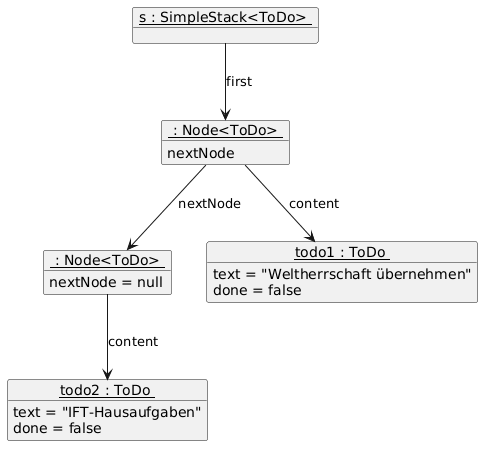
\includegraphics[width=0.7\linewidth]{a5}

\label{fig:a5}
\end{figure}


\end{document}
